\documentclass[10pt]{beamer}
\usepackage[utf8]{inputenc}

\usepackage{multirow,rotating}
\usepackage{color}
\usepackage{hyperref}
\usepackage{tikz-cd}
\usepackage{array}
\usepackage{siunitx}
\usepackage{graphicx}
\usepackage{tcolorbox}
\usepackage{mathtools,nccmath}%
\usepackage{etoolbox, xparse} 
\usetheme{CambridgeUS}
\usecolortheme{dolphin}

% set colors
\definecolor{myNewColorA}{RGB}{186,12,47} %Bulldog Red
\definecolor{myNewColorB}{RGB}{0,163,173} % Lake Herrick Blue
\definecolor{myNewColorC}{RGB}{0, 0,0} %Arch Black
\definecolor{myNewColorD}{RGB}{255,255,255} % Chapel Bell White
\setbeamercolor*{palette primary}{bg=myNewColorC}
\setbeamercolor*{palette secondary}{bg=myNewColorB, fg = white}
\setbeamercolor*{palette tertiary}{bg=myNewColorA, fg = white}
\setbeamercolor*{titlelike}{fg=myNewColorA}
\setbeamercolor*{title}{bg=myNewColorA, fg = white}
\setbeamercolor*{item}{fg=myNewColorA}
\setbeamercolor*{caption name}{fg=myNewColorA}
\setbeamercolor{alerted text}{fg=myNewColorB}
\setbeamercolor{alerted text}{bg=myNewColorC}
\setbeamercolor{block title}{bg=myNewColorA,fg=myNewColorC}
\setbeamercolor{block body}{bg=myNewColorD}
\usefonttheme{professionalfonts}
\usepackage{natbib}
\usepackage{hyperref}
%------------------------------------------------------------
% \titlegraphic{\includegraphics[height=0.75cm]{ua_eng_logo.png}} 

% logo of my university


\titlegraphic{%

\includegraphics[width=3.0cm]{UGAlogo.png}
}

\setbeamerfont{title}{size=\large}
\setbeamerfont{subtitle}{size=\small}
\setbeamerfont{author}{size=\small}
\setbeamerfont{date}{size=\footnotesize}
\setbeamerfont{institute}{size=\footnotesize}
\title[3PG: The Basics]{3PG: The Basics}%title
%\subtitle{ }%%subtitle
\author[Quentin Boccaleri]{Quentin Boccaleri\inst{1}}%%authors

\institute[UGA]{The University of Georgia\inst{1}}
\date[\textcolor{white}{Precision Silviculture, 2025}]
{Precision Silviculture\\
Aug XX, 2025}

%------------------------------------------------------------
%This block of commands puts the table of contents at the 
%beginning of each section and highlights the current section:
%\AtBeginSection[]
%{
%  \begin{frame}
%    \frametitle{Contents}
%    \tableofcontents[currentsection]
%  \end{frame}
%}
\AtBeginSection[]{
  \begin{frame}
  \vfill
  \centering
  \begin{beamercolorbox}[sep=8pt,center,shadow=true,rounded=true]{title}
    \usebeamerfont{title}\insertsectionhead\par%
  \end{beamercolorbox}
  \vfill
  \end{frame}
}
% ------Contents below------
%------------------------------------------------------------

\begin{document}

\frame{\titlepage}

\begin{frame}
\frametitle{Outline}
\tableofcontents
\end{frame}

%------------------------------------------------------------
\section{What is 3PG?} 
\begin{frame}
\frametitle{The Big Picture}
\begin{center}
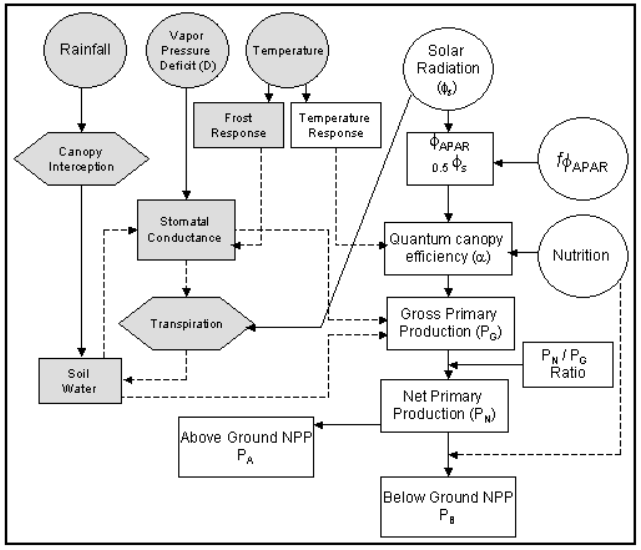
\includegraphics[width=8.0cm]{3PG.png.png}
\end{center}
\end{frame}

\begin{frame}
\frametitle{The Big Picture}
\begin{center}
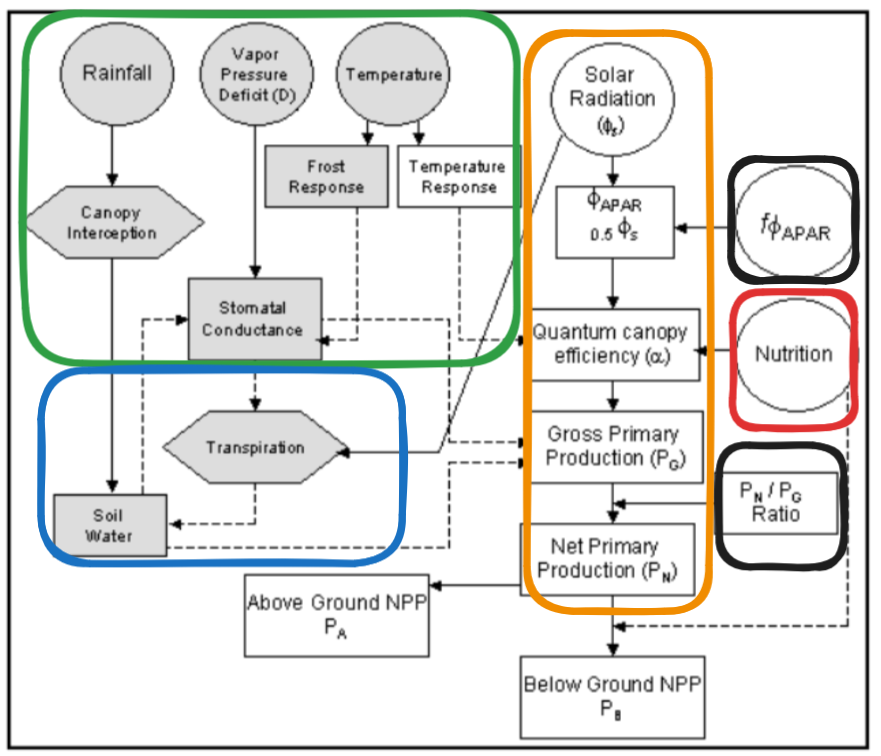
\includegraphics[width=8.0cm]{3PG2.png}
\end{center}
\end{frame}

\section{The Engine of 3PG} 
\begin{frame}
\begin{enumerate}
\item 3PG begins with taking \textbf{incoming solar radiation}, and converting it into \textbf{Photosynthetically Active Radiation (PAR)}.
\begin{center}
$PAR = 0.5(GR)$
\end{center}
\begin{center}
\textit{Where PAR and GR are in MJ per m per day.}
\end{center}
\vspace{3mm}
\item PAR must then be converted into \textbf{GPP}.
\begin{center}
$P_g = \alpha_c(1-e^{-kL})Q_0$
\end{center}
\begin{center}
\textit{Where $P_g$ is GPP (MJ per m per day), $\alpha_c$ is canopy quantum efficiency, $(1-e^{-kL})Q_0$ is Beer's Law.}
\end{center}
\vspace{3mm}
\item GPP is then converted into \textbf{NPP} using a constant fraction of 0.47.
\end{enumerate}
\end{frame}

\begin{frame}{Beer's Law}
\begin{enumerate}
\item Beer's law describes the absorption of light as it passes through a medium. 
\item Equation $(1-e^{-kL})Q_0$ describes the interception of light from the canopy based on LAI (l). k is an absorption coefficient. $Q_0$ is the amount of light before it passes through the canopy.   
\end{enumerate}
\begin{center}
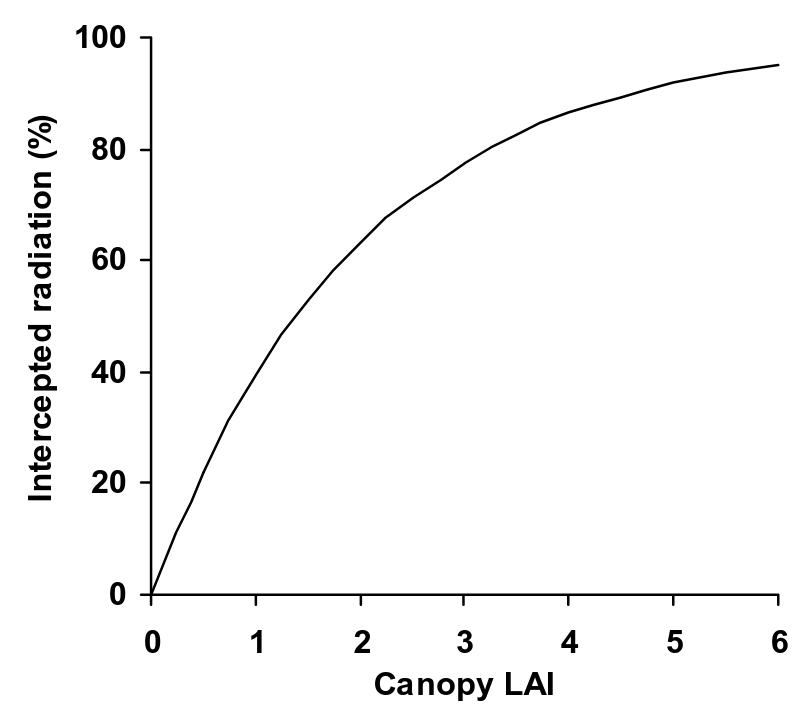
\includegraphics[width=5.0cm]{beer.png}    
\end{center}
\end{frame}

\begin{frame}{Canopy Quantum Efficiency}
    
\end{frame}
    



\section{Conclusion}
\begin{frame}{Conclusion}
\begin{enumerate}[(1)]
\item Point 1 
\vspace{3mm}
\vspace{3mm}
\item Point 2 
\vspace{3mm}
\vspace{3mm}

• Point 2a
\end{enumerate}
\end{frame}

\section{Contact Information}  
\begin{frame}

\textcolor{myNewColorC}{\huge{\centerline{Thank you!}}}
\vspace*{0.5cm}

\textcolor{myNewColorA}{\Large{\centerline{E-mail: GoDawgs@uga.edu}}}

\end{frame}

\end{document}



